\documentclass[12pt,a4paper,twoside]{article}
\usepackage{microtype}
\usepackage{graphicx}
\usepackage[utf8]{inputenc}
\usepackage[T1]{fontenc}
\usepackage{amsmath,amsfonts,amssymb}
\usepackage{subcaption}
\usepackage{float}
\usepackage{caption}
\usepackage{booktabs}
\usepackage{pgfplots}
\usepackage{tikz}
\pgfplotsset{compat=1.18}
\usepackage{array}
\usepackage{multirow}
\usepackage{capt-of}
\usepackage{longtable}
\usepackage{tabularx}
\usepackage{wrapfig}
\usepackage{siunitx}
\usepackage{multicol}
\usepackage{listings}
\usepackage{qrcode}
\usepackage{mfirstuc}
\usepackage[most]{tcolorbox}
\usepackage{xcolor}

\definecolor{OxfordBlue}{HTML}{002147}
\definecolor{noteblue}{RGB}{0, 102, 204}
\definecolor{notebg}{RGB}{240, 245, 255}
\definecolor{darkred}{RGB}{139, 0, 0}

\usepackage[a4paper]{geometry}
\geometry{
  top=1in,
  bottom=1in,
  left=1.25in,
  right=1in
}

\usepackage{fancyhdr}
\pagestyle{fancy}
\renewcommand{\headrulewidth}{0pt}
\fancyhf{}

\fancyfoot[RO]{
    \footnotesize
    \textcolor{gray}{\copyright{} 2026--2027 Maroua Mezhoud}
    \quad
    \textcolor{gray!60!black}{\rule[-0.5pt]{0.5pt}{8pt}}
    \quad
    \textcolor{black}{\thepage}
}

\fancyfoot[LE]{
    \footnotesize
    \textcolor{black}{\thepage}
    \quad
    \textcolor{gray!60!black}{\rule[-0.5pt]{0.5pt}{8pt}}
    \quad
    \textcolor{gray}{\copyright{} 2026--2027 Maroua Mezhoud}
}

\newtcolorbox{mynotebox}{
    enhanced,
    breakable,
    colback=notebg,
    colframe=notebg,
    borderline west={3pt}{0pt}{noteblue},
    arc=4pt,
    outer arc=4pt,
    left=15pt,
    right=10pt,
    top=10pt,
    bottom=10pt
}

\definecolor{simpink}{RGB}{236, 72, 153}
\definecolor{simpurple}{RGB}{147, 82, 214}
\definecolor{simblue}{RGB}{59, 130, 246}

\definecolor{simpinkbg}{RGB}{255, 243, 249}
\definecolor{simpurplebg}{RGB}{247, 242, 255}
\definecolor{simbluebg}{RGB}{240, 246, 255}

\newtcolorbox{simbox}{
    enhanced,
    breakable,
    colback=simpurplebg,
    colframe=simpurple,
    arc=6pt,
    outer arc=6pt,
    boxrule=1.6pt,
    frame style={left color=simpink, middle color=simpurple, right color=simblue},
    interior style={left color=simpinkbg, middle color=simpurplebg, right color=simbluebg},
    left=12pt,
    right=10pt,
    top=8pt,
    bottom=8pt
}

\usepackage{hyperref}
\hypersetup{
    colorlinks=true,
    linkcolor=black,
    urlcolor=OxfordBlue
}

\usepackage{wallpaper}
\usepackage{background}
\backgroundsetup{
  scale=4,
  color=gray!50,
  opacity=0.2,
  angle=55,
  contents={}
}
\usepackage{eso-pic}

\definecolor{codegray}{rgb}{0.45,0.45,0.45}
\definecolor{codebackground}{rgb}{0.98,0.98,0.97}
\definecolor{keywordcolor}{rgb}{0.20,0.35,0.60}
\definecolor{commentcolor}{rgb}{0.65,0.40,0.55}
\definecolor{stringcolor}{rgb}{0.60,0.20,0.70}

\lstset{
    language=Python,
    basicstyle=\ttfamily\small,
    backgroundcolor=\color{codebackground},
    keywordstyle=\color{keywordcolor}\bfseries,
    commentstyle=\color{commentcolor}\itshape,
    stringstyle=\color{stringcolor},
    numbers=left,
    numberstyle=\tiny\color{codegray},
    stepnumber=1,
    numbersep=10pt,
    frame=single,
    framerule=0.5pt,
    rulecolor=\color{gray!30},
    breaklines=true,
    showstringspaces=false,
    tabsize=4,
    captionpos=b,
    xleftmargin=15pt
}



\begin{document} %===============================================

%------------------------------------------------------------------
% PAGE DE GARDE
%------------------------------------------------------------------
\begin{titlepage}

\ThisCenterWallPaper{1}{images/Front-Page-BG.pdf}

\centering

\begin{flushleft}
    
\includegraphics[width=0.18\textwidth]{images/footer-logo.png}
\end{flushleft}

\vspace{1cm}

{\Large \textbf{Mohamed El Bachir El Ibrahimi University of Bordj Bou Arréridj} \par}

{\large Faculty of Science and Technology \par}

{\large Department of Materials Science \par}

{\large Third-Year Undergraduate Programme (LMD)\par}
{\large Radiation Physics\par}

{\large Course: Nuclear Physics \par}

\vspace*{\fill}
{\Huge \textbf{Practical Work N\textsuperscript{o}\,1} \\ \textbf{Simulation and Analysis of Rutherford Scattering of Alpha Particles} \par}

\vspace*{\fill}

  {\large \textbf{Submitted by:} \\ Maroua Mezhoud \par}

\vspace{1cm}

    {\large \textbf{Supervised by:} \\ Dr. Khalfallah Farid \par}
    {Group: 2 \par}

\vspace{2cm}

    {\large Date of submission: \today \par}

    {\large Academic Year: 2026--2027 \par}

\vfill

\end{titlepage}


\newpage

\pagestyle{fancy}
\pagenumbering{arabic}
\setcounter{page}{1}

%------------------------------------------------------------------
% 1. INTRODUCTION
%------------------------------------------------------------------
\section{Introduction}
In 1909, Geiger and Marsden, under Rutherford's direction, directed
$\alpha$ particles at a thin gold foil. Thomson's model predicted only small
deflections, yet most particles passed straight through, while a few were
scattered at large angles and some were even backscattered. Rutherford
concluded in 1911 that the positive charge and almost all the mass of the atom
are concentrated in a tiny, dense nucleus. The scattering is governed by the
Coulomb repulsion between the $\alpha$ particle (charge $2e$) and the nucleus
(charge $Ze$). In this practical work, we use a simulation to determine the
minimum distance of approach $d_{\min}$, show that it varies linearly with $Z$,
recover the kinetic energy $E_c$ of the $\alpha$ particles, and compare the
simulated $\theta(b)$ with Rutherford's formula.

%------------------------------------------------------------------
% 2. SIMULATION
%------------------------------------------------------------------
\section{Simulation of the Experiment}
The simulation was performed for alpha particles interacting with a gold
nucleus ($Z=79$), with a kinetic energy
\[
E = 6\,\mathrm{MeV}.
\]
Figure~\ref{fig:z79} shows the simulation interface, displaying the scattering trajectories of alpha particles and the curve $\theta$ as a function of the impact
parameter $b$. The minimum distance of approach obtained from the simulation
is $d_{\min} = 37.92\,\mathrm{fm}$.

\begin{figure}[H]
    \centering
    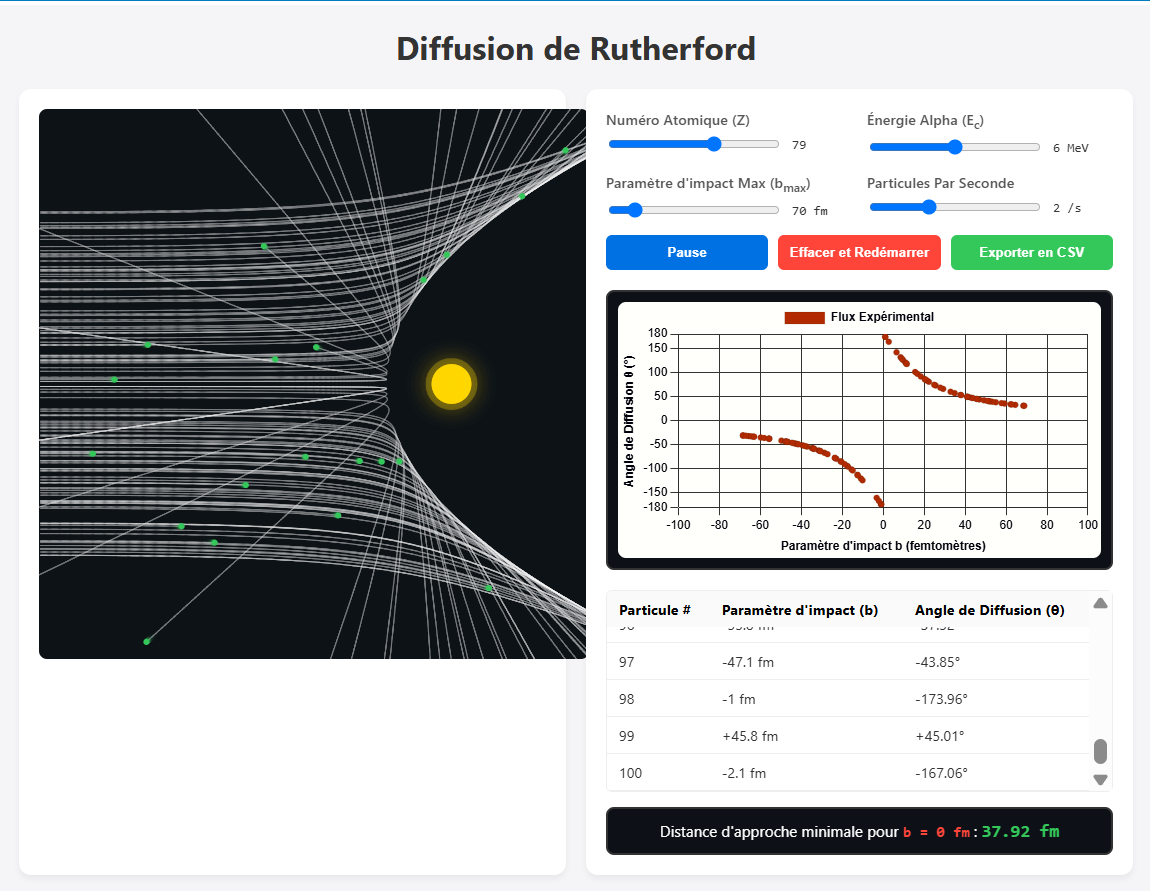
\includegraphics[width=0.85\textwidth]{images/image.png}
    \caption{Simulation interface for gold ($Z=79$) with $E=6\,\mathrm{MeV}$, showing scattering trajectories and the minimum distance $d_{\min}$.}
    \label{fig:z79}
\end{figure}

The simulation was performed using the online Rutherford scattering tool, which is available \href{https://sites.google.com/view/khalfar/expphys/rutherford}{here}.

%------------------------------------------------------------------
% 3. DISTANCE MINIMALE
%------------------------------------------------------------------
\section{Minimum Distance of Approach}

For a head-on collision, the alpha particle approaches the target nucleus
until its initial kinetic energy is entirely converted into electrostatic
potential energy. At the minimum distance of approach $d_{\min}$, the kinetic
energy is momentarily zero.

By conservation of energy:
\begin{equation}
E_c = \frac{k(2e)(Ze)}{d_{\min}}.
\end{equation}

Therefore,
\begin{equation}
E_c = \frac{2kZe^2}{d_{\min}}.
\end{equation}

Rearranging this expression gives:
\begin{equation}
d_{\min} = \frac{2ke^2}{E_c}\,Z.
\end{equation}

Defining the constant
\begin{equation}
C_\alpha = \frac{2ke^2}{E_c},
\end{equation}
we obtain the required linear relationship:
\begin{equation}
\boxed{d_{\min} = C_\alpha Z}.
\end{equation}

Thus, for a fixed kinetic energy, the minimum distance of approach is
directly proportional to the atomic number $Z$ of the target nucleus.


%------------------------------------------------------------------
% 4. CALCUL DE Ec
%------------------------------------------------------------------
\section{Calculation of the Kinetic Energy $E_c$ of the Alpha Particles}

The alpha-particle kinetic energy was kept constant at \(E = 6\,\mathrm{MeV}\).
Simulations were performed for four atomic numbers, \(Z = 50, 60, 70,\) and \(80\).
For each value of \(Z\), the minimum distance of approach, \(d_{\min}\), was
recorded from the simulator's output field (the simulator does not display it
on the plotted curve) and is reported in Table~\ref{tab:dm-z}. The corresponding
simulation results are presented in Figure~\ref{fig:rutherford-comparison}.

\begin{table}[H]
    \centering
    \begin{tabular}{|c|c|c|c|}
        \hline
        $Z$ & $d_m$ simulated (fm) & $d_m$ theoretical (fm) & Relative error (\%) \\
        \hline
        50 & 24.00 & 24.00 & 0 \\
        60 & 28.80 & 28.80 & 0 \\
        70 & 33.60 & 33.60 & 0 \\
        80 & 38.40 & 38.40 & 0 \\
        \hline
    \end{tabular}
    \caption{Minimum distance of approach $d_m$ for different values of $Z$
    ($E=6\,\mathrm{MeV}$). The theoretical values are computed from
    $d_m = \dfrac{2ke^2}{E_c}\,Z = \dfrac{2\times1.44}{6}\,Z$
    with $ke^2 = 1.44\,\mathrm{MeV\,fm}$.}
    \label{tab:dm-z}
\end{table}



\begin{figure}[H]
    \centering

    \begin{subfigure}[b]{0.48\textwidth}
        \centering
        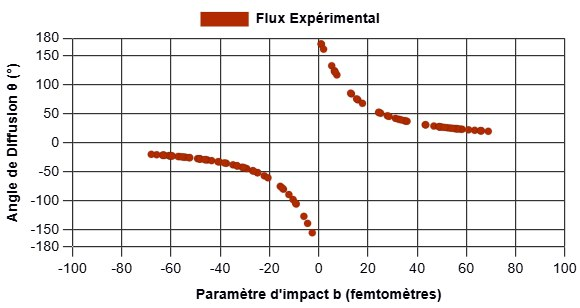
\includegraphics[width=\textwidth]{images/graphes/z=50.jpg}
        \caption{$Z=50$ ($d_{\min} = 24.00\text{ fm}$)}
        \label{fig:rutherford-z50}
    \end{subfigure}
    \hfill
    \begin{subfigure}[b]{0.48\textwidth}
        \centering
        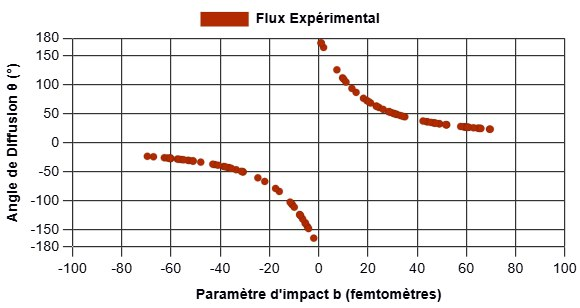
\includegraphics[width=\textwidth]{images/graphes/z=60.jpg}
        \caption{$Z=60$ ($d_{\min} = 28.80\text{ fm}$)}
        \label{fig:rutherford-z60}
    \end{subfigure}

    \vspace{0.5cm}

    \begin{subfigure}[b]{0.48\textwidth}
        \centering
        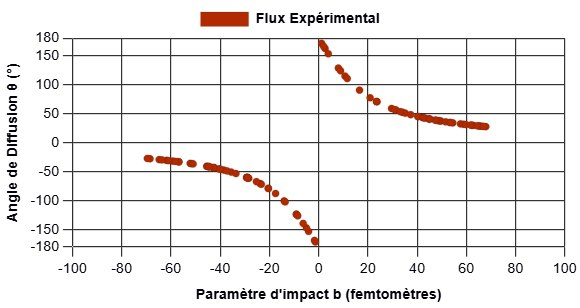
\includegraphics[width=\textwidth]{images/graphes/z=70.jpg}
        \caption{$Z=70$ ($d_{\min} = 33.60\text{ fm}$)}
        \label{fig:rutherford-z70}
    \end{subfigure}
    \hfill
    \begin{subfigure}[b]{0.48\textwidth}
        \centering
        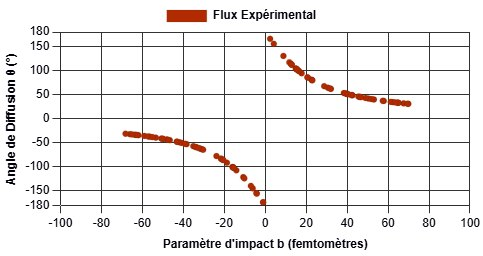
\includegraphics[width=\textwidth]{images/graphes/z=80.jpg}
        \caption{$Z=80$ ($d_{\min} = 38.40\text{ fm}$)}
        \label{fig:rutherford-z80}
    \end{subfigure}

    \caption{Simulation curves for $Z=50, 60, 70, 80$ at $E=6\,\mathrm{MeV}$.}
    \label{fig:rutherford-comparison}
\end{figure}

The experimental data are plotted to verify the linear relationship between \(d_{\min}\) and \(Z\).
 

\begin{figure}[H]
    \centering
    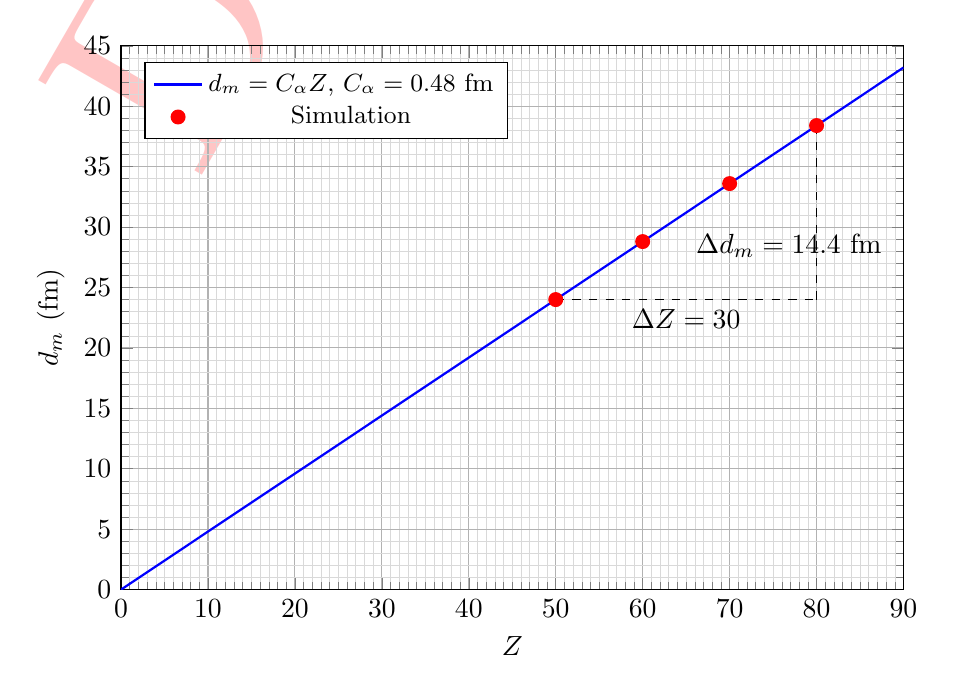
\begin{tikzpicture}
    \begin{axis}[
        width=0.95\textwidth,
        height=0.7\textwidth,
        xlabel={$Z$},
        ylabel={$d_m$ (fm)},
        xmin=0, xmax=90,
        ymin=0, ymax=45,
        xtick distance=10,
        ytick distance=5,
        minor x tick num=9,
        minor y tick num=4,
        grid=both,
        major grid style={thin, gray!60},
        minor grid style={very thin, gray!30},
        legend pos=north west,
        legend style={font=\small, fill=white},
    ]
    % Droite d_m = C_alpha * Z
    \addplot[blue, thick, domain=0:90] {0.48*x};
    \addlegendentry{$d_m = C_\alpha Z$, $C_\alpha = 0.48$ fm}

    % Points de simulation
    \addplot[only marks, mark=*, red, mark size=2.5pt]
        coordinates {(50,24) (60,28.8) (70,33.6) (80,38.4)};
    \addlegendentry{Simulation}

    % Triangle de pente
\draw[dashed, black] (axis cs:50,24) -- (axis cs:80,24)
    node[midway, below] {$\Delta Z = 30$};
\draw[dashed, black] (axis cs:80,24) -- (axis cs:80,38.4)
    node[pos=0.5, xshift=-10pt, yshift=-12pt] {$\Delta d_m = 14.4$ fm};
    \end{axis}
    \end{tikzpicture}
    \caption{Minimum distance of approach $d_m$ versus atomic number $Z$
($E=6\,\mathrm{MeV}$). The slope of the line gives $C_\alpha$.}
    \label{fig:dm-vs-z}
\end{figure}

The slope of the line in Figure~\ref{fig:dm-vs-z} is
\begin{equation}
C_\alpha = \frac{\Delta d_m}{\Delta Z} = \frac{38.40 - 24.00}{80 - 50}
= \frac{14.40}{30} = 0.48\ \mathrm{fm}.
\end{equation}
\begin{equation}
E_c = \frac{2ke^2}{C_\alpha} = \frac{2\times 1.44}{0.48}
= 6.00\ \mathrm{MeV}.
\end{equation}
\noindent \textbf{Note:} Using $k = 8.99 \times 10^{9} \text{ N}\cdot\text{m}^2/\text{C}^2$ and $e = 1.60 \times 10^{-19} \text{ C}$:
\begin{equation*}
ke^2 = \frac{(8.99 \times 10^9) \times (1.60 \times 10^{-19})^2}{(1.602 \times 10^{-13} \text{ J/MeV}) \times (10^{-15} \text{ m/fm})} \approx 1.44 \text{ MeV}\cdot\text{fm}
\end{equation*}
The relative error with respect to the imposed energy ($6\,\mathrm{MeV}$) is
$0\,\%$, which confirms the linear law $d_m = C_\alpha Z$.




%------------------------------------------------------------------
% 5. ANGLE DE DIFFUSION (BONUS)
%------------------------------------------------------------------
\section{Scattering Angle}

\subsection*{Method 1: Plot with Python (Matplotlib)}

The scattering angle $\theta$ depends on the impact parameter $b$, the atomic
number $Z$ of the target nucleus, and the initial kinetic energy $E_c$ of the
alpha particles. According to Rutherford's scattering theory, the theoretical
scattering angle is given by
\begin{equation}
\theta(b)=\frac{180}{\pi}\,2\arctan
\left(\frac{k e^2 Z}{E_c b}\right),
\label{eq:rutherford-angle}
\end{equation}
where $k e^2=1.44\,\mathrm{MeV\,fm}$, $E_c$ is the kinetic energy of the alpha
particles, and $b$ is the impact parameter expressed in femtometers (fm). The
angle $\theta$ is expressed in degrees.

For a gold nucleus, the parameters are
\[
Z=79,\qquad E_c=6\,\mathrm{MeV}.
\]

The simulation data are exported as a CSV file containing the 100 pairs
$(b,\theta)$. These data are plotted together with the theoretical curve
given by Equation~\eqref{eq:rutherford-angle} in Figure~\ref{fig:scattering-angle}.

\begin{figure}[H]
    \centering
    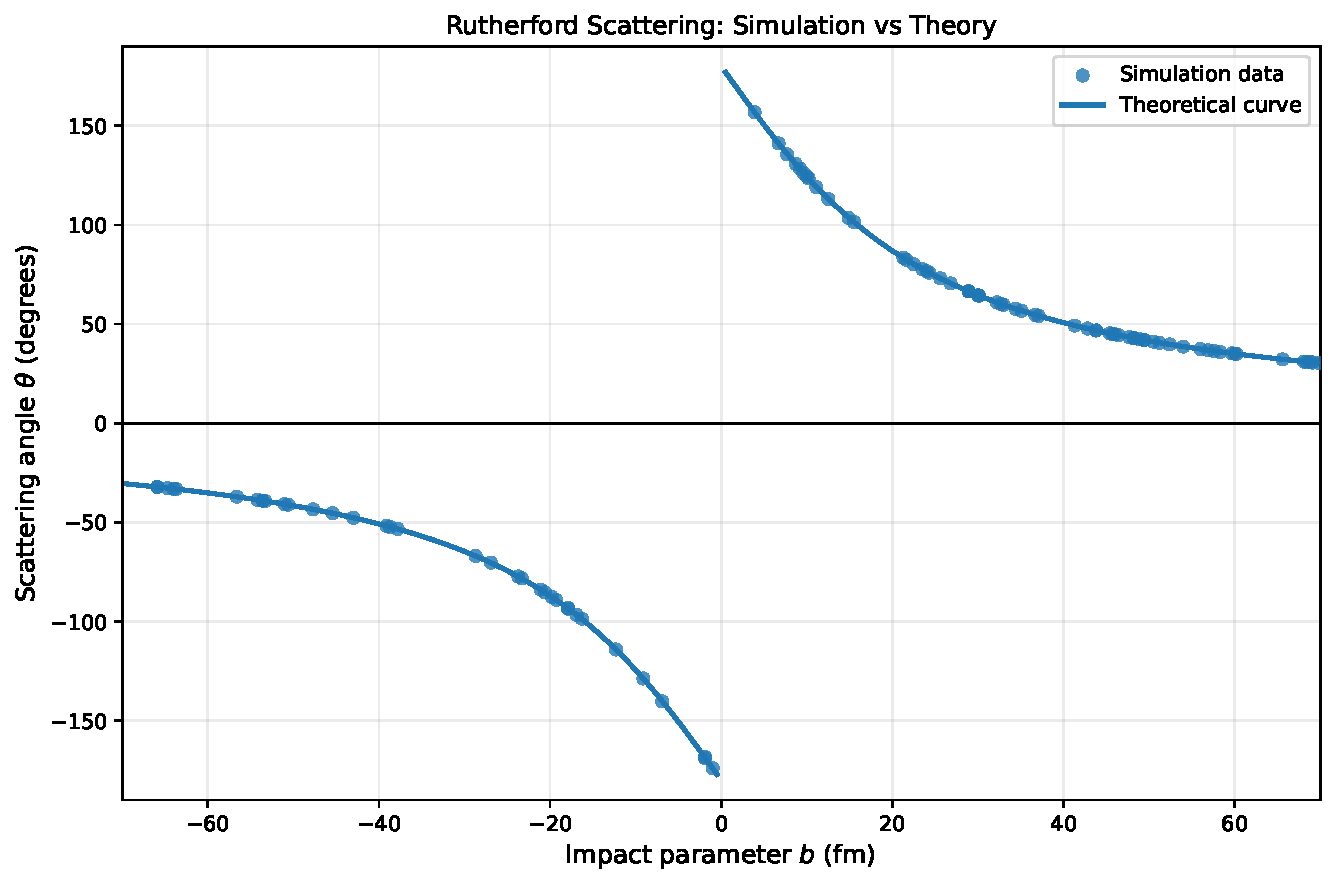
\includegraphics[width=0.85\textwidth]{images/graphes/rutherford_scattering.pdf}
    \caption{Comparison between the simulated and theoretical Rutherford
    scattering angles for gold ($Z=79$) at $E_c=6\,\mathrm{MeV}$.}
    \label{fig:scattering-angle}
\end{figure}

The comparison allows us to assess the agreement between the simulation
results and Rutherford's theoretical prediction. The scattering angle
decreases as the impact parameter increases: small values of $b$
(near head-on collisions) give large deflection angles, while large values of
$b$ give almost undeviated trajectories.

\subsubsection*{Python Code for the Scattering Angle}

The following script processes the exported simulation data and plots it
against Rutherford's theoretical formula:

\begin{lstlisting}[caption={Python script for processing and plotting Rutherford scattering data.}, label={lst:rutherford-code}]

import numpy as np
import pandas as pd
import matplotlib.pyplot as plt
from pathlib import Path

# --------------------------------------------------
# 1. Read the simulation data
# --------------------------------------------------
data = pd.read_csv("data.csv")

b = data["Impact_Parameter_b_fm"].to_numpy()
theta_sim = data["Diffusion_Theta_Degrees"].to_numpy()

# --------------------------------------------------
# 2. Define the theoretical Rutherford scattering law
# Z = 79, Ec = 6 MeV, k*e^2 = 1.44 MeV.fm
# --------------------------------------------------
Z = 79
Ec = 6.0
ke2 = 1.44

def theta_theory(b):
    return np.degrees(
        2 * np.arctan((ke2 * Z) / (Ec * b))
    )

# Split the curve at b = 0 to avoid division by zero
b_negative = np.linspace(-70, -0.5, 1000)
b_positive = np.linspace(0.5, 70, 1000)

# --------------------------------------------------
# 3. Plot simulation points and theoretical curves
# --------------------------------------------------
fig, ax = plt.subplots(figsize=(9, 6))

ax.scatter(
    b, theta_sim,
    s=28,
    alpha=0.8,
    label="Simulation data",
    zorder=3
)

line, = ax.plot(
    b_negative,
    theta_theory(b_negative),
    linewidth=2,
    label="Theoretical curve"
)

ax.plot(
    b_positive,
    theta_theory(b_positive),
    linewidth=2,
    color=line.get_color()
)

ax.set_xlabel(r"Impact parameter $b$ (fm)", fontsize=12)
ax.set_ylabel(r"Scattering angle $\theta$ (degrees)", fontsize=12)

ax.set_title("Rutherford Scattering: Simulation vs Theory")
ax.set_xlim(-70, 70)
ax.set_ylim(-190, 190)

ax.axhline(0, color="black", linewidth=0.7)
ax.grid(True, alpha=0.25)
ax.legend()
fig.tight_layout()

# --------------------------------------------------
# 4. Save the figures
# --------------------------------------------------
output_dir = Path("images/graphes")
output_dir.mkdir(parents=True, exist_ok=True)

fig.savefig(
    output_dir / "rutherford_scattering.png",
    dpi=300,
    bbox_inches="tight"
)

fig.savefig(
    output_dir / "rutherford_scattering.pdf",
    bbox_inches="tight"
)

print(f"Number of simulation points: {len(data)}")
print("Figures saved successfully in the images/graphes folder.")

plt.show()

\end{lstlisting}


\subsection*{Method 2: Plot with TikZ (PGFPlots)}

The same data are plotted again using TikZ for a publication-quality vector figure.

\begin{figure}[H]
\centering
\begin{tikzpicture}
\begin{axis}[
    width=0.85\textwidth,
    height=0.6\textwidth,
    xlabel={Impact Parameter $b$ (fm)},
    ylabel={Scattering Angle $\theta$ (Degrees)},
    grid=major,
    grid style={gray!35, dashed},
    minor tick num=1,
    tick style={black, thin},
    label style={font=\large},
    tick label style={font=\small},
    legend style={font=\small, at={(0.97,0.95)}, anchor=north east, cells={anchor=west}},
    every axis plot/.append style={thick},
    mark size=1.5pt,
]
% Courbe théorique : theta(b) = 2*atan(ke2*Z/(Ec*b)), ke2*Z/Ec = 1.44*79/6 = 18.96
\addplot[red, thick, no marks, domain=0.3:70, samples=200] {2*atan(18.96/x)};
\addlegendentry{Theoretical curve}

\addplot[red, thick, no marks, domain=-70:-0.3, samples=200, forget plot] {2*atan(18.96/x)};

\addplot+[only marks, mark=*, blue] 
    table[x=Impact_Parameter_b_fm, y=Diffusion_Theta_Degrees, col sep=comma] {data.csv};
\addlegendentry{Experimental data}

\end{axis}
\end{tikzpicture}
\caption{Relationship between impact parameter and scattering angle.}
\label{fig:diffusion_data}
\end{figure}


%------------------------------------------------------------------
% Conclusion
%------------------------------------------------------------------
\section{Conclusion}
This practical work demonstrated the linear dependence of the minimum distance of approach ($d_{\min}$) on the atomic number ($Z$), allowing the initial kinetic energy of the alpha particles to be recovered as ($E_c=6.00\text{ MeV}$). The comparison between the simulated and theoretical scattering angles also showed excellent agreement with Rutherford's scattering law for gold. These results illustrate how numerical simulation can be used to test theoretical predictions in nuclear physics.


%------------------------------------------------------------------
%  SOURCE CODE AND REPRODUCIBILITY
%------------------------------------------------------------------
\section{Source Code and Reproducibility}

\begin{mynotebox}
\begin{center}
    \begin{minipage}{0.7\textwidth}
        \centering
        To ensure transparency and reproducibility, \textcolor{darkred}{all Python source code, CSV data files, TikZ figures, graphics, and the full \LaTeX\ source code for this document} are publicly available on my GitHub repository.\
        \href{https://github.com/Maroua-Mezhoud/Physics-Lab-Reports/tree/main/Atomic-physics-Lap-Report/PW1-Rutherford\%20Scattering}{\texttt{GitHub Repository}}
    \end{minipage}%
    \begin{minipage}{0.2\textwidth}
        \centering
        \qrcode[height=2cm]{https://github.com/Maroua-Mezhoud/Physics-Lab-Reports/tree/main/Atomic-physics-Lap-Report/PW1-Rutherford\%20Scattering}
    \end{minipage}
    \\[1mm]
    \footnotesize \textit{Scan or click to access the repository}
\end{center}
\end{mynotebox}

%------------------------------------------------------------------
%  INTERACTIVE WEB SIMULATION
%------------------------------------------------------------------
\section{Interactive Web Simulation}

\begin{simbox}
\begin{center}
    \begin{minipage}{0.72\textwidth}
        As an addition, I recreated the Rutherford scattering simulation using \textbf{JavaScript} with AI assistance, and published it on our \textbf{Physics Club} website.
        \\[2mm]
        \href{https://maroua-mezhoud.github.io/physics-club/simulations/rutherford-scattering/index.html}{\textcolor{simpink}{\textbf{Try the Web Simulation $\rightarrow$}}}
        
    \end{minipage}%
    \hfill
    \begin{minipage}{0.22\textwidth}
        \centering
        \qrcode[height=1.8cm]{https://maroua-mezhoud.github.io/physics-club/simulations/rutherford-scattering/index.html}
    \end{minipage}
    \\[1mm]
    \footnotesize \textit{\textcolor{gray}{Scan or click to open the simulation}}
\end{center}
\end{simbox}



%------------------------------------------------------------------
\newpage
\thispagestyle{empty}
\backgroundsetup{contents={\copyright{} 2026--2027 Maroua Mezhoud}}
\BgThispage
\null

\newpage

\end{document}